\scanpage{54}
d'où $\varepsilon^F_{\Phi',\Phi}$. Cette fois on aura
\[
\left\{\begin{aligned}
\varepsilon^{\deleted{\unsure{S}}F}_{\Phi',\Phi}\circ\varepsilon^F_{\Phi,\Phi'}&=\mathrm{id}_{F_{\Phi'}}\qquad\text{et de }=\\
\varepsilon^F_{\Phi,\Phi'}\circ\varepsilon^F_{\Phi',\Phi}&=\mathrm{id}_{F_\Phi}
\end{aligned}\right.
\]

Soit enfin $a$ une arête commune à $\Phi,\Phi'$
i.e. $a\in\unsure{\mathcal P|P|\mathfrak P}_2(S)$. Alors $S\smallsetminus\{a\}=\alpha_\Phi\amalg\alpha_{\Phi'}$, où $\alpha_\Phi$ est
formé des deux éléments \inserted{$u$}\deleted{\unsure{$s$}} de $S\smallsetminus\{a\}$ tels que
$(S\smallsetminus\{a\})\cup\{u\}\in\Phi$, et \unsure{item|idem|itou} pour $\alpha_{\Phi'}$. On a bij. can.
\figure{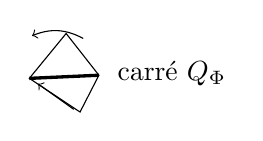
\begin{tikzpicture}[scale=.57]
\draw (0,.1)--(.82,1.1)--(1.55,.17)--(1.13,-.65)--cycle;
\draw[very thick] (0,.1)--(1.55,.17);
\draw[->] (1.2,.99) to[bend right=25] (.06,1.05);
\draw[->] (.99,-.59)--(.19,-.02);
\node[right] at (1.75,.2) {carré $Q_\Phi$};
\end{tikzpicture}}
\[
\begin{aligned}
\widetilde A_{\Phi,a}&\simeq a\wedge\alpha_\Phi\quad\inserted{(\simeq\omega(Q_\Phi))}\qquad\text{et de }=\\
\widetilde A_{\Phi',a}&\simeq a\wedge\alpha_{\Phi'}
\end{aligned}
\]
donc
\[
\widetilde A_{\Phi,a}\wedge\widetilde A_{\Phi',a}\simeq\alpha_\Phi\wedge\alpha_{\Phi'}\simeq a
\]
\margin{(NB on a $a\wedge a_\Phi\wedge a_{\Phi'}\overset{\mathrm{can}}{=}1$ à cause de l'orientation canonique de l'ens $S$ comme de $\{\Phi,\Phi'\}$).}

Donc choisir une bijection entre $\widetilde A_{\Phi,a}$ et $\widetilde A_{\Phi',a}$, \deleted{\unsure{revient}}
à choisir un élément de $a$, \inserted{i.e. une orientation de l'arête $a$}.
Donc on n'a pas
vraiment ici de bijection canonique au niveau
de $\widetilde A_\Phi$ et $\widetilde A_{\Phi'}$ comme annoncé. Ainsi, on
trouve une bijection
\[
\deleted{\unsure{\varepsilon}}\varepsilon^{\vec A}_{\Phi',\Phi}:
\overrightarrow{\widetilde A}_\Phi\xrightarrow{\sim}\overrightarrow{\widetilde A}_{\Phi'}
\qquad\text{et de $=$ en sens inv.}
\]
satisfaisant cette fois
\[
\left\{\begin{aligned}
\varepsilon^{\vec A}_{\Phi',\Phi}\,\varepsilon^{\vec A}_{\Phi,\Phi'}&=\mathrm{id}_{\overrightarrow{\widetilde A}_{\Phi'}}\qquad\text{et de }=\\
\varepsilon^{\vec A}_{\Phi,\Phi'}\,\varepsilon^{\vec A}_{\Phi',\Phi}&=\mathrm{id}_{\overrightarrow{\widetilde A}_\Phi}
\end{aligned}\right.
\]
% slanted
\margin{\uline{NB} $\overrightarrow{\widetilde A}_\Phi\simeq\operatorname{Rep}^{+}\deleted{\unsure{\Phi}}\inserted{(S,A,\Phi)}$, $\overrightarrow{\widetilde A}_{\Phi'}\simeq\operatorname{Rep}^{+}\inserted{(S,A,\Phi')}$}

En résumé : Pour les dodécaèdres \deleted{\unsure{duaux|des}}\inserted{$D,D'$} duaux
des icosaèdres $\widetilde{(S,A,\Phi)}=I$ et $\widetilde{(S,A,\Phi')}=I'$, \deleted{il y a}\inserted{on}
peut considérer $D,D'$ \unsure{pointés|portés|précisés} par \uline{le $=$} ens
de sommets (le choix de l'identification \unsure{en|ne}
dépendant \unsure{pas|par} du choix d'un $\Phi\in\{\Phi,\Phi'\}$),
mais l'analogue au niveau $I,I'$ n'est
pas vrai : le choix d'une identification des
sommets . $S(I)\simeq S(I')$ dépend du choix de $I$ ou $I'$.
% archive sheet number: 53
